% Copyright(c) Spenego Software LLC

\chapter{Obidos - Introductory Concepts}

Obidos is a web based Application that allows users to store and share digital artifacts securely without any out of band means.
These artifacts can be confidential information, similar to passwords or credit card details or bank account information.
Or, it can be information that the User wants to keep securely in one place so that they are easily accessible when needed.
One example of this is the warranty information or service contract details of an equipment or machine.
In Obidos, information can be shared to groups of users or to individual users. 
Any information shared with a group/user is visible only to that group/user. It is also possible to revoke sharing.
The duration of sharing can be controlled by setting an expiration date. After the expiration date, 
the shared information will not be visible to the recipient.

\section{Items}
In Obidos, an Item is defined as a secure encrypted representation of a digital artifact. Such an Item can be stored in Obidos. The encryption is done in such a way that the Item can be decrypted only with a passphrase that is private to the User.
Every Item has a name. It is possible to search for an Item using its name.
\subsection{Fields and Values}
Each Item is made up of field(s) and value(s) that corresponds to the details of the artifact it represents.

For example, an Item named 'Xyz contract' can have multiple fields like 'Customer number' with value '5643291',
'Tech support phone\#' with value '888-5555-1111' and 'Contract expiration' as '31 Dec, 2025'.

\begin{figure}[H]
\centering
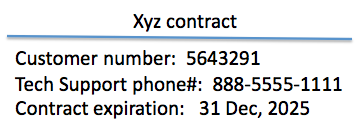
\includegraphics[width=70mm]{common/Figure-0.png}
\caption{Item}
\label{fig: Figure}
\end{figure}

\subsection{Shareable and Private Items}
There are two types of Items; Shareable and Private.
A Private Item cannot be shared with others while a Shareable Item can be shared.

%\subsubsection{Notes}
\section{Notes}
A Note is a special type of Item. It is similar to a sticky note (or postit note). 
A Note is a secure encrypted representation of its sticky note equivalent.
Every Note has a name. A Note also has a field that stores the content of the Note. 
Obidos provides a main menu option to manage Notes as 'standalone' Items since Notes are very commonly used, 
Standalone Notes are free standing Notes and can be created as Private or Shareable. Notes are the only free standing Items in Obidos.

\begin{figure}[H]
\centering
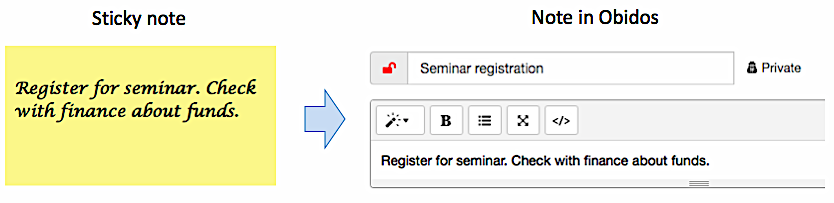
\includegraphics[width=120mm]{common/Note.png}
\caption{Note}
\label{fig: Figure}
\end{figure}

%\subsection{Containers}
\section{Containers}
Items stored inside Obidos can be organized into Containers. Each Container has a name.
For example, a Container named 'Personal Items' can be created to hold Items that are personal in nature.

There are two types of Containers; Private and Shareable.
Shareable Containers can be shared with others while Private Containers cannot be shared. 
By default, every user gets a Private Container called 'Private' and a Shareable Container called 'Public'. 

Each Container holds the Items stored in it.
Placing of an Item in a Container is dictated by the type of the Container and the type of the Item.

Private Containers can hold only Private Items. A Shareable Item cannot be placed in a Private Container.
Shareable Containers can hold both Shareable and Private Items (see Figure 1.3).

\begin{figure}[H]
\centering
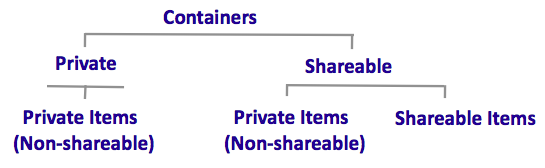
\includegraphics[width=90mm]{common/Figure-1.png}
\caption{Containers}
\label{fig: Figure}
\end{figure}

When a Shareable Container is shared with others, only Shareable Items inside the Container will be visible to them.
Private Items inside that Shareable Container will be completely hidden from others.

As an example, a Private Container named 'Personal Items' can be created to contain 3 Private Items 
named 'Bank Account', 'Cloud Account', and 'Procurement Card'. Note that in this case all the three Items will be Private
because a Private Container can hold only Private Items.

In addition to having a name, each Item is made up of field(s) and value(s).
For example, in the 'Personal Items' container, the 'Bank Account' Item can have a field 
'Account\#' with value '87399901".
In case the Routing number of the bank has to be stored, another field 'Routing\#'
can be added with its value '3452327'. (See figure 1.4)

\begin{figure}[H]
\centering
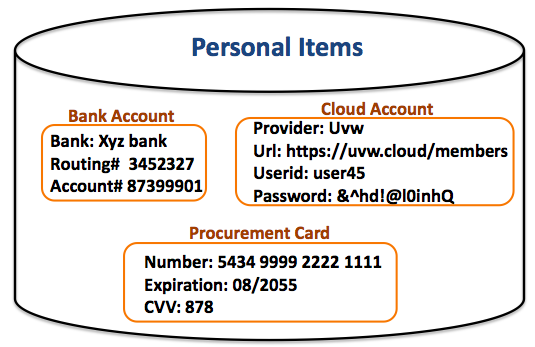
\includegraphics[width=80mm]{common/PersonalItems.png}
\caption{Private Container}
\label{fig: Figure}
\end{figure}

A Shareable Container named 'Lab Accounts' can be used to hold Shareable Items that has names 'xyz customer support' and 'Web Console'.
'Lab Accounts' Container may also hold a Private Item 'Database Account'.
When 'Lab Accounts' is shared to others, they will see the Items 'xyz customer support' and 'Web Console', but
will not see the Item 'Database Account'. (See figure 1.5)

\begin{figure}[H]
\centering
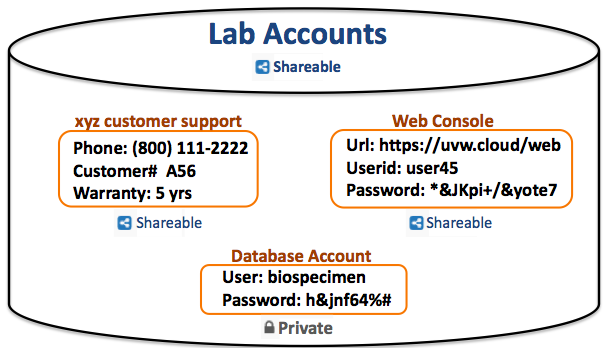
\includegraphics[width=80mm]{common/Lab-Accounts.png}
\caption{Shareable Container}
\label{fig: Figure}
\end{figure}

Users have permissions to create/modify Containers and Items. The distinction between standalone Notes and Containerized Items is visually represented in the following figure.

\begin{figure}[H]
\centering
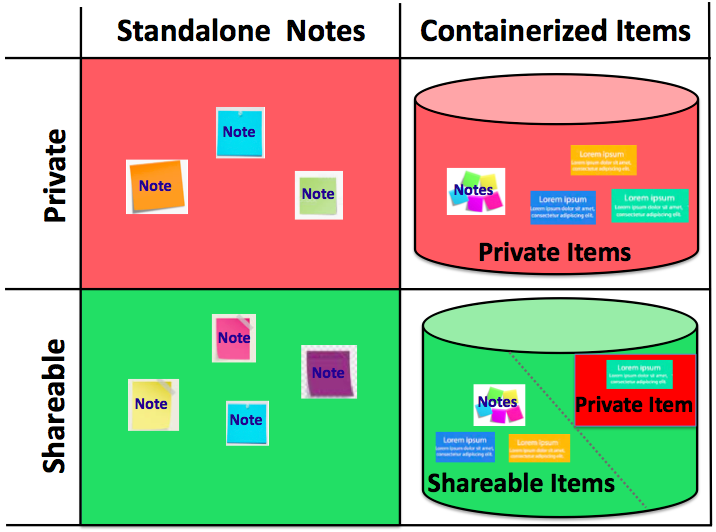
\includegraphics[width=80mm]{common/Standalone-Container.png}
\caption{Standalone Notes and Containerized Items}
\label{fig: Figure}
\end{figure}

\section{Templates}
There are various Items that follow a common format. Such formats can be captured as Templates.
Templates provide common structures for often used Items. A Template has the pre-defined fields of the Item.
These Templates can be used as a guide to create instances of Items in a Container.
When using a Template to create an Item, the User has to just fill in the values for the predefined fields.
Templates can be Global or Personal. Global Templates are available to all users.
Obidos provides a number of predefined Global Templates. 

For example, a Template called 'Cloud Account' can have the following fields:
  \newline \tab \tab url, username, password, email

When a user uses the 'Cloud Account' Template to create an Item called 'Web Server', values for the fields
url, username, password and email have to be supplied by the User (see following Figure).

\begin{figure}[H]
\centering
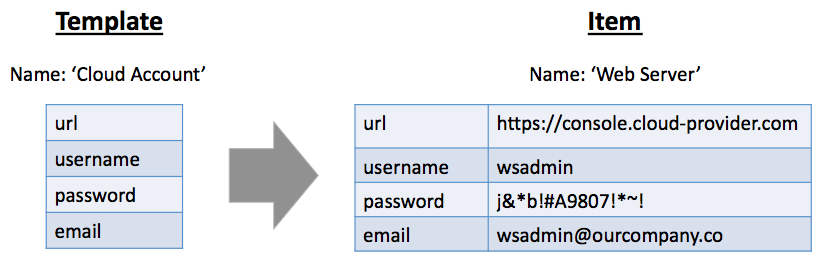
\includegraphics[scale=0.5]{common/Template-Item.png}
\caption{Instantiation of an Item from a Template}
\label{fig: Figure}
\end{figure}

Every user has permissions to create/modify Personal Templates.
However, creation/modification of Global Templates requires special permission.
The administrator can grant a user permission to create/modify Global Templates.
Users can also copy a Global Template into their Personal Templates and modify it to suit their purpose.

\section{Groups}
A set of users can be organized into a Group. The Group can have a name. It is possible to share an entity with a Group.
This makes it easy to share with a collection of users; especially if sharing is done to the same Group for multiple entities.

\section{Features}
Note that all features of Obidos are discussed in the guides. However, only the features that are licensed will be 
available in the instance.
